\section{Servicios de Documento (Backend)}
Dentro de este paquete se encuentra la clase principal de interaccion con el sistema, basicamente es lo unico que una 
View conoceria.

La clase \texttt{WordService} es el backend principal y punto de entrada a todo el sistema. Los servicios que expone 
son los que se detallaron en la secci�n de Arquitectura:
\begin{itemize}
  \item Agregar un documento
  \item Realizar una consulta
  \item Reproducir un documento
\end{itemize}

\subsection{WordService}

\paragraph{Interacciones}
Se encarga de instanciar el Indexador, el Crawler, el servicio de persistencia de sonidos (utilizando un Trie), la
librer�a de documentos y el SearchEngine, y orquestar las relaciones entre ellos.

\paragraph{Metodos}
Expone los metodos principales para agregar, buscar y reproducir documentos. Que son delegados a los demas objetos.

\paragraph{Conexion con View}
La conexion con View se hace explicitamente en los metodos par agregar y reproducir a traves de una interfase (IWordsRecordConnector), de esta manera el servicio no conoce especificamente que view lo utiliza.

\subsection{Crawler}
El crawler es una entidad bastante simple que se encarga de agregar documentos al sistema.

\paragraph{Agregar un documento al sistema}
El proceso de agregar un documento, consta de los siguientes pasos:

\begin{enumerate}
\item Agregar el documento a la Librer�a de Documentos.
\item Iniciar una sesi�n con el Indexador.
\item Pasar el documento al Parser que ira retornando las distintas frases.
\item Cada frase se pasa por el discriminador de stop words que devuelve solo los terminos relevantes.
\item Se indexan los terminos relevantes en el Indexador.
\item Una vez terminadas las frases del documentos, se cierra la sesi�n con el indexador.
\item Se devuelve el lexico completo del documento (incluyendo las stopwords).
\end{enumerate}

A continuaci�n se muestra un diagrama de secuencia de este proceso.

\begin{figure}[!htp]
\centering
\makebox[\textwidth]{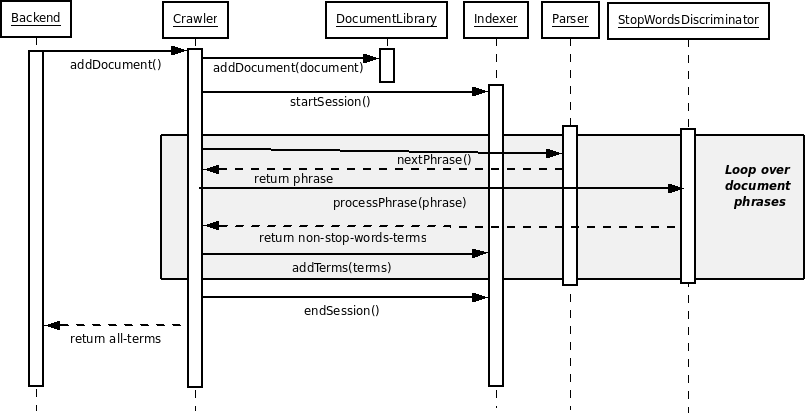
\includegraphics[scale=0.5,natwidth=20pt,natheight=10pt]{img/crawler.png}}
\caption{Diagrama de secuencia: Proceso de agregar un documento al sistema.} 
\end{figure}
